\documentclass[11pt]{article}
\usepackage[margin=1in]{geometry}
\usepackage{enumitem}
\usepackage{hyperref}
\usepackage{graphicx}
\usepackage{array}
\usepackage{multicol}
\usepackage{enumitem}
\usepackage{longtable}
\usepackage{titlesec}
\usepackage{amsmath}
\begin{document}

\begin{center}
    \large \textbf{Sri Sivasubramaniya Nadar College of Engineering, Chennai} \\
    (An autonomous Institution affiliated to Anna University) \\
    \vspace{0.3cm}
\end{center}
\begin{table}[!h]
\renewcommand{\arraystretch}{1.5}
\resizebox{\textwidth}{!}{%
\begin{tabular}{|l|cll|}
\hline
Degree \& Branch     & \multicolumn{1}{c|}{B.E.   Computer Science \& Engineering} & \multicolumn{1}{l|}{Semester}        & V                                        \\ \hline
Subject Code \& Name & \multicolumn{3}{c|}{ICS1512 \& Machine Learning Algorithms Laboratory}                                                                              \\ \hline
Academic year       & \multicolumn{1}{c|}{2025-2026 (Odd)}                        & \multicolumn{1}{c|}{Batch:2023-2028} & \multicolumn{1}{c|}{\textbf{Due date:}} \\ \hline
\end{tabular}%
}
\end{table}
\begin{center}
 \textbf{
{\Large Experiment 2: Loan Amount Prediction using Linear Regression}
}
\end{center}
\textbf{\large Aim:} To predict the loan amount sanctioned to users using Linear Regression on historical data, and analyze model performance using visual and statistical metrics. 

\vspace{0.5cm}
\noindent
\textbf{\large Libraries used:} 
\begin{itemize}
    \item Pandas - for data handling
    \item numpy - for numerical operations
    \item matplotlib.pyplot and seaborn - for visualization
    \item sklearn - for model building and evaluation
\end{itemize}

\vspace{0.5cm}
\noindent
\textbf{\large Objective:} To build a linear regression model using Scikit-learn to predict the loan amount, perform exploratory data analysis, visualize model performance, and interpret results.

\vspace{0.5cm}
\noindent
\textbf{\large Mathetical/theoritical description: } The linear regression model expresses the relationship between the input features and the predicted output as:

\[
y = \beta_0 + \beta_1 x_1 + \beta_2 x_2 + \dots + \beta_n x_n + \epsilon
\]

Where:
\begin{itemize}
    \item $y$ is the predicted loan amount,
    \item $x_i$ are the input features (e.g., income, credit score, etc.),
    \item $\beta_i$ are the coefficients (weights) learned by the model,
    \item $\epsilon$ is the error term (residual).
\end{itemize}
 
\vspace{0.5cm}
\noindent
\textbf{\large CODE}:
\begin{verbatim}
import pandas as pd
import numpy as np
import matplotlib.pyplot as plt
import seaborn as sns
import google.colab.drive as drive
from sklearn.model_selection import train_test_split, cross_val_score, KFold
from sklearn.linear_model import LinearRegression
from sklearn.metrics import mean_absolute_error, mean_squared_error, r2_score
from sklearn.preprocessing import StandardScaler

# 1. Load Dataset
drive.mount('/content/drive')
df = pd.read_csv('/content/drive/MyDrive/Colab Notebooks/ML LAB SEM 5/train.csv')
print(df.head())

## Drop non-informative identifiers
df.drop(columns=["Customer ID", "Name", "Property ID"], inplace=True)

# Handle missing values (optional: use better imputation)
df.dropna(inplace=True)

# Define target variable
target = "Loan Sanction Amount (USD)"
X = df.drop(columns=[target])
y = df[target]

# Encode categorical variables
categorical_cols = X.select_dtypes(include=["object"]).columns
X = pd.get_dummies(X, columns=categorical_cols, drop_first=True)

# Normalize numerical features
scaler = StandardScaler()
X_scaled = scaler.fit_transform(X)

# 3. EDA
# a. Loan Amount Distribution Plot
sns.histplot(df["Loan Sanction Amount (USD)"], kde=True, color="skyblue")
plt.title("Loan Sanction Amount Distribution")
plt.xlabel("Loan Sanction Amount (USD)")
plt.ylabel("Frequency")
plt.grid(True)
plt.show()

# b. Correlation Heatmap (only for numeric columns)
numeric_df = df.select_dtypes(include=["number"])  # selects only numeric columns
plt.figure(figsize=(12, 8))
sns.heatmap(numeric_df.corr(), annot=True, cmap="coolwarm", fmt=".2f", linewidths=0.5)
plt.title("Correlation Heatmap of Numeric Features")
plt.show()
\end{verbatim}
\textbf{OUTPUT}
\begin{center}
  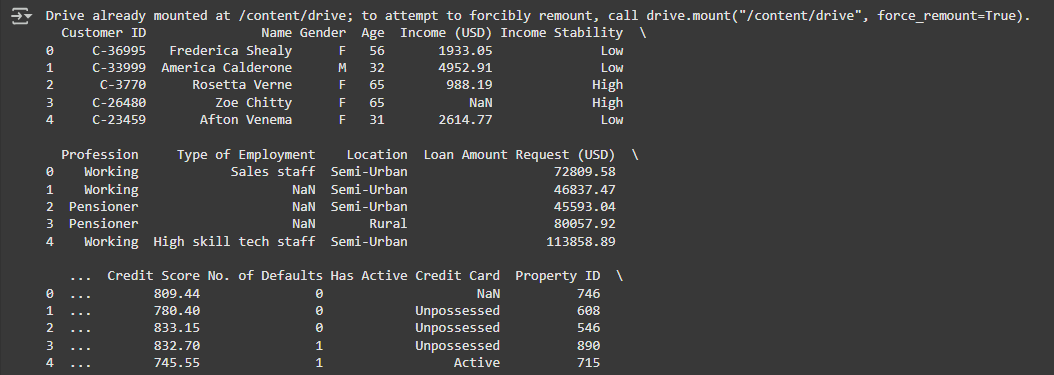
\includegraphics[width=0.8\textwidth]{sc1.png}
\end{center}
\begin{center}
  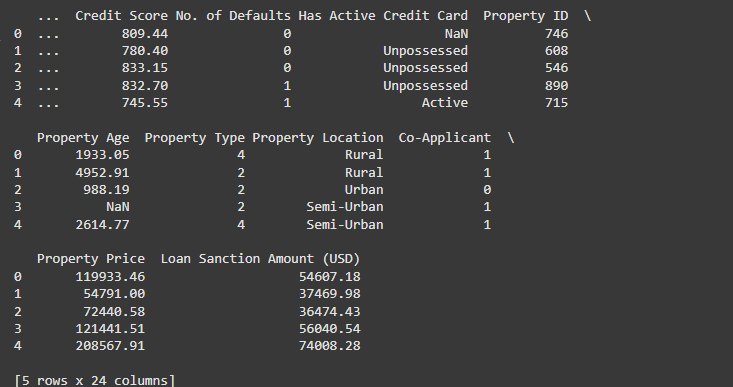
\includegraphics[width=0.8\textwidth]{sc2.png}
\end{center}
\begin{center}
  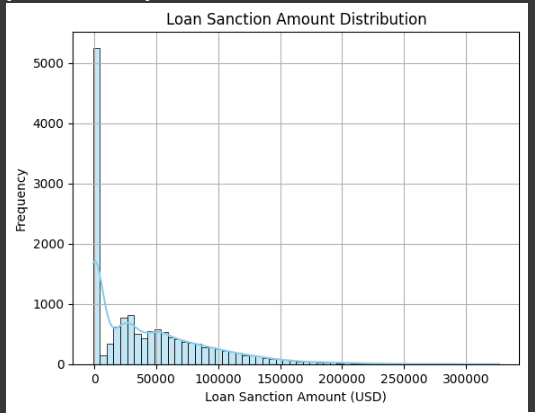
\includegraphics[width=0.8\textwidth]{sc3.png}
\end{center}
\begin{center}
  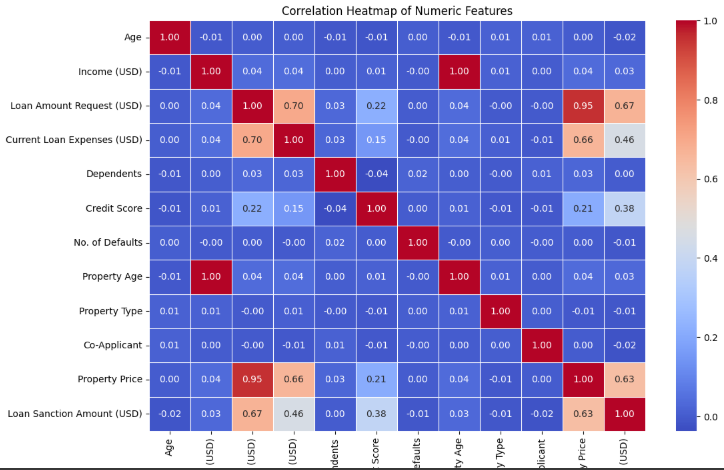
\includegraphics[width=0.8\textwidth]{sc4.png}
\end{center}

\begin{verbatim}
---------------------------------------------------------------------------------------------
# 4. Train-test Split
X_train, X_test, y_train, y_test = train_test_split(X_scaled, y, test_size=0.2, random_state=42)

# 5. Train Model
model = LinearRegression()
model.fit(X_train, y_train)

# 6. Evaluate
y_pred = model.predict(X_test)

mae = mean_absolute_error(y_test, y_pred)
mse = mean_squared_error(y_test, y_pred)
rmse = np.sqrt(mse)
r2 = r2_score(y_test, y_pred)
adj_r2 = 1 - (1 - r2) * (len(y) - 1) / (len(y) - X.shape[1] - 1)

print(f"MAE: {mae}, MSE: {mse}, RMSE: {rmse}, R2: {r2}, Adj R2: {adj_r2}")
\end{verbatim}
\textbf{OUTPUT}
\begin{verbatim}
MAE: 25323.793500422737, 
MSE: 1195267145.5071688, 
RMSE: 34572.63579056663, 
R2: 0.47512320259332885, 
Adj R2: 0.47375943210040017 
---------------------------------------------------------------------------------------------
# 7. Visualizations
plt.scatter(y_test, y_pred)
plt.xlabel("Actual loan amount")
plt.ylabel("Predicted loan anount")
plt.title("Actual vs Predicted Loan Amount")
plt.show()

residuals = y_test - y_pred
sns.residplot(x=y_pred, y=residuals, lowess=True)
plt.title("Residual Plot")
plt.show()

plt.bar(x=X.columns, height=model.coef_)
plt.xticks(rotation=90)
plt.title("Feature Coefficients")
plt.show()
\end{verbatim}
\textbf{OUTPUT}
\begin{center}
  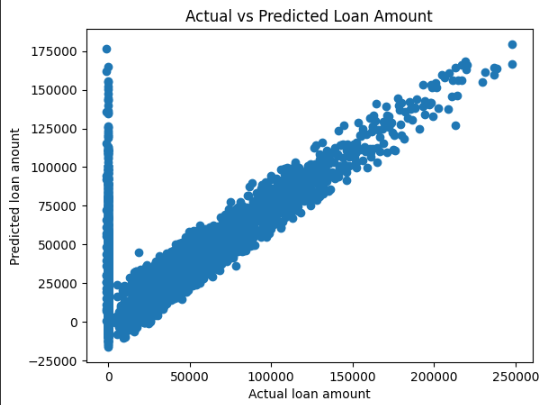
\includegraphics[width=0.8\textwidth]{sc5.png}
\end{center}
\begin{center}
  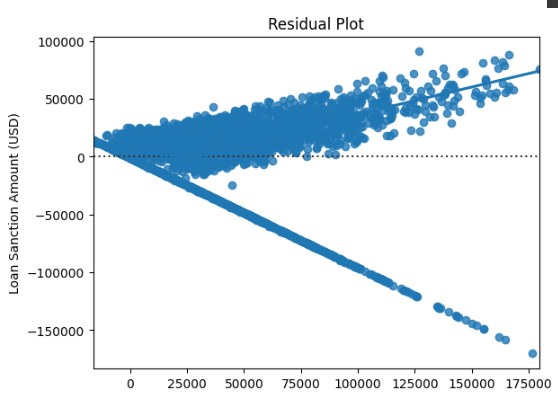
\includegraphics[width=0.8\textwidth]{sc6.png}
\end{center}
\begin{center}
  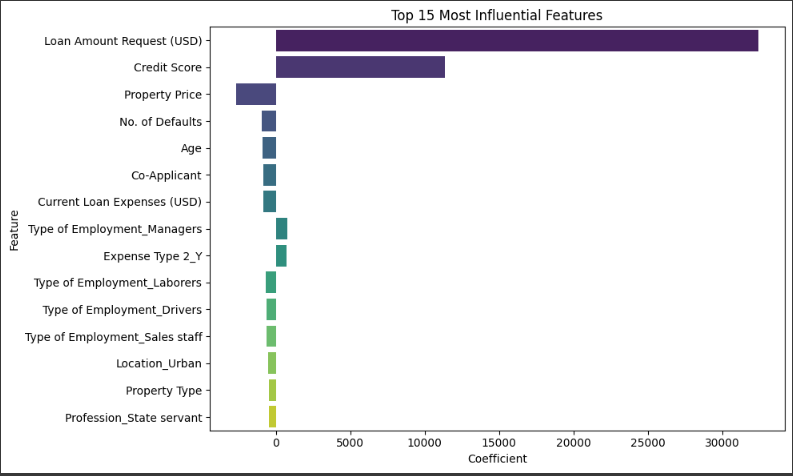
\includegraphics[width=0.8\textwidth]{sc7.png}
\end{center}

\vspace{0.5cm}
\noindent
\textbf{\large Results and Discussions:} 

\vspace{0.5cm}
\noindent



\vspace{0.5cm}
\noindent
\end{document}
